% Options for packages loaded elsewhere
\PassOptionsToPackage{unicode}{hyperref}
\PassOptionsToPackage{hyphens}{url}
%
\documentclass[
]{article}
\usepackage{amsmath,amssymb}
\usepackage{iftex}
\ifPDFTeX
  \usepackage[T1]{fontenc}
  \usepackage[utf8]{inputenc}
  \usepackage{textcomp} % provide euro and other symbols
\else % if luatex or xetex
  \usepackage{unicode-math} % this also loads fontspec
  \defaultfontfeatures{Scale=MatchLowercase}
  \defaultfontfeatures[\rmfamily]{Ligatures=TeX,Scale=1}
\fi
\usepackage{lmodern}
\ifPDFTeX\else
  % xetex/luatex font selection
\fi
% Use upquote if available, for straight quotes in verbatim environments
\IfFileExists{upquote.sty}{\usepackage{upquote}}{}
\IfFileExists{microtype.sty}{% use microtype if available
  \usepackage[]{microtype}
  \UseMicrotypeSet[protrusion]{basicmath} % disable protrusion for tt fonts
}{}
\makeatletter
\@ifundefined{KOMAClassName}{% if non-KOMA class
  \IfFileExists{parskip.sty}{%
    \usepackage{parskip}
  }{% else
    \setlength{\parindent}{0pt}
    \setlength{\parskip}{6pt plus 2pt minus 1pt}}
}{% if KOMA class
  \KOMAoptions{parskip=half}}
\makeatother
\usepackage{xcolor}
\usepackage[margin=1in]{geometry}
\usepackage{color}
\usepackage{fancyvrb}
\newcommand{\VerbBar}{|}
\newcommand{\VERB}{\Verb[commandchars=\\\{\}]}
\DefineVerbatimEnvironment{Highlighting}{Verbatim}{commandchars=\\\{\}}
% Add ',fontsize=\small' for more characters per line
\usepackage{framed}
\definecolor{shadecolor}{RGB}{248,248,248}
\newenvironment{Shaded}{\begin{snugshade}}{\end{snugshade}}
\newcommand{\AlertTok}[1]{\textcolor[rgb]{0.94,0.16,0.16}{#1}}
\newcommand{\AnnotationTok}[1]{\textcolor[rgb]{0.56,0.35,0.01}{\textbf{\textit{#1}}}}
\newcommand{\AttributeTok}[1]{\textcolor[rgb]{0.13,0.29,0.53}{#1}}
\newcommand{\BaseNTok}[1]{\textcolor[rgb]{0.00,0.00,0.81}{#1}}
\newcommand{\BuiltInTok}[1]{#1}
\newcommand{\CharTok}[1]{\textcolor[rgb]{0.31,0.60,0.02}{#1}}
\newcommand{\CommentTok}[1]{\textcolor[rgb]{0.56,0.35,0.01}{\textit{#1}}}
\newcommand{\CommentVarTok}[1]{\textcolor[rgb]{0.56,0.35,0.01}{\textbf{\textit{#1}}}}
\newcommand{\ConstantTok}[1]{\textcolor[rgb]{0.56,0.35,0.01}{#1}}
\newcommand{\ControlFlowTok}[1]{\textcolor[rgb]{0.13,0.29,0.53}{\textbf{#1}}}
\newcommand{\DataTypeTok}[1]{\textcolor[rgb]{0.13,0.29,0.53}{#1}}
\newcommand{\DecValTok}[1]{\textcolor[rgb]{0.00,0.00,0.81}{#1}}
\newcommand{\DocumentationTok}[1]{\textcolor[rgb]{0.56,0.35,0.01}{\textbf{\textit{#1}}}}
\newcommand{\ErrorTok}[1]{\textcolor[rgb]{0.64,0.00,0.00}{\textbf{#1}}}
\newcommand{\ExtensionTok}[1]{#1}
\newcommand{\FloatTok}[1]{\textcolor[rgb]{0.00,0.00,0.81}{#1}}
\newcommand{\FunctionTok}[1]{\textcolor[rgb]{0.13,0.29,0.53}{\textbf{#1}}}
\newcommand{\ImportTok}[1]{#1}
\newcommand{\InformationTok}[1]{\textcolor[rgb]{0.56,0.35,0.01}{\textbf{\textit{#1}}}}
\newcommand{\KeywordTok}[1]{\textcolor[rgb]{0.13,0.29,0.53}{\textbf{#1}}}
\newcommand{\NormalTok}[1]{#1}
\newcommand{\OperatorTok}[1]{\textcolor[rgb]{0.81,0.36,0.00}{\textbf{#1}}}
\newcommand{\OtherTok}[1]{\textcolor[rgb]{0.56,0.35,0.01}{#1}}
\newcommand{\PreprocessorTok}[1]{\textcolor[rgb]{0.56,0.35,0.01}{\textit{#1}}}
\newcommand{\RegionMarkerTok}[1]{#1}
\newcommand{\SpecialCharTok}[1]{\textcolor[rgb]{0.81,0.36,0.00}{\textbf{#1}}}
\newcommand{\SpecialStringTok}[1]{\textcolor[rgb]{0.31,0.60,0.02}{#1}}
\newcommand{\StringTok}[1]{\textcolor[rgb]{0.31,0.60,0.02}{#1}}
\newcommand{\VariableTok}[1]{\textcolor[rgb]{0.00,0.00,0.00}{#1}}
\newcommand{\VerbatimStringTok}[1]{\textcolor[rgb]{0.31,0.60,0.02}{#1}}
\newcommand{\WarningTok}[1]{\textcolor[rgb]{0.56,0.35,0.01}{\textbf{\textit{#1}}}}
\usepackage{graphicx}
\makeatletter
\def\maxwidth{\ifdim\Gin@nat@width>\linewidth\linewidth\else\Gin@nat@width\fi}
\def\maxheight{\ifdim\Gin@nat@height>\textheight\textheight\else\Gin@nat@height\fi}
\makeatother
% Scale images if necessary, so that they will not overflow the page
% margins by default, and it is still possible to overwrite the defaults
% using explicit options in \includegraphics[width, height, ...]{}
\setkeys{Gin}{width=\maxwidth,height=\maxheight,keepaspectratio}
% Set default figure placement to htbp
\makeatletter
\def\fps@figure{htbp}
\makeatother
\setlength{\emergencystretch}{3em} % prevent overfull lines
\providecommand{\tightlist}{%
  \setlength{\itemsep}{0pt}\setlength{\parskip}{0pt}}
\setcounter{secnumdepth}{-\maxdimen} % remove section numbering
\ifLuaTeX
  \usepackage{selnolig}  % disable illegal ligatures
\fi
\IfFileExists{bookmark.sty}{\usepackage{bookmark}}{\usepackage{hyperref}}
\IfFileExists{xurl.sty}{\usepackage{xurl}}{} % add URL line breaks if available
\urlstyle{same}
\hypersetup{
  pdftitle={Lab 6},
  pdfauthor={Cameron Adams},
  hidelinks,
  pdfcreator={LaTeX via pandoc}}

\title{Lab 6}
\author{Cameron Adams}
\date{Math 241, Week 8}

\begin{document}
\maketitle

\begin{Shaded}
\begin{Highlighting}[]
\CommentTok{\# Put all necessary libraries here}
\FunctionTok{library}\NormalTok{(tidyverse)}
\FunctionTok{library}\NormalTok{(leaflet)}
\FunctionTok{library}\NormalTok{(tidycensus)}
\FunctionTok{library}\NormalTok{(tidyverse)}
\FunctionTok{library}\NormalTok{(tidycensus)}
\FunctionTok{library}\NormalTok{(flextable)}
\FunctionTok{library}\NormalTok{(sf)}
\FunctionTok{library}\NormalTok{(tigris)}
\FunctionTok{library}\NormalTok{(tmap)}
\FunctionTok{library}\NormalTok{(RColorBrewer)}
\end{Highlighting}
\end{Shaded}

\hypertarget{due-friday-march-22nd-at-830am}{%
\subsection{Due: Friday, March 22nd at
8:30am}\label{due-friday-march-22nd-at-830am}}

\hypertarget{goals-of-this-lab}{%
\subsection{Goals of this lab}\label{goals-of-this-lab}}

\begin{itemize}
\tightlist
\item
  Practice creating static and interactive choropleth maps.
\end{itemize}

\hypertarget{problem-1-mapping-bike-rides-in-portland}{%
\subsubsection{Problem 1: Mapping Bike Rides in
Portland}\label{problem-1-mapping-bike-rides-in-portland}}

For this problem we will return to the biketown dataset.

\begin{enumerate}
\def\labelenumi{\alph{enumi}.}
\tightlist
\item
  Grab the code from activity 9, Problem 1 to read the data directly
  from Biketown's API- make sure to keep the longitude and latitude of
  the start of each ride (\texttt{StartLatitude},
  \texttt{StartLongitude}).
\end{enumerate}

\begin{Shaded}
\begin{Highlighting}[]
\NormalTok{biketown\_data }\OtherTok{\textless{}{-}} \FunctionTok{bind\_rows}\NormalTok{(readr}\SpecialCharTok{::}\FunctionTok{read\_csv}\NormalTok{(}\StringTok{"https://s3.amazonaws.com/biketown{-}tripdata{-}public/2017\_01.csv"}\NormalTok{),}
\NormalTok{                           readr}\SpecialCharTok{::}\FunctionTok{read\_csv}\NormalTok{(}\StringTok{"https://s3.amazonaws.com/biketown{-}tripdata{-}public/2017\_07.csv"}\NormalTok{),}
\NormalTok{                           readr}\SpecialCharTok{::}\FunctionTok{read\_csv}\NormalTok{(}\StringTok{"https://s3.amazonaws.com/biketown{-}tripdata{-}public/2017\_11.csv"}\NormalTok{)) }\SpecialCharTok{\%\textgreater{}\%}
  

  \FunctionTok{select}\NormalTok{(StartDate, StartTime, EndDate, EndTime, Distance\_Miles,}
\NormalTok{         BikeID, StartLongitude, StartLatitude )}
\end{Highlighting}
\end{Shaded}

\begin{enumerate}
\def\labelenumi{\alph{enumi}.}
\setcounter{enumi}{1}
\tightlist
\item
  Create an interactive map of the start point of the rides using the
  \texttt{leaflet} package. Make sure to include a legend and a title.
  What do you notice about the distribution of rides?
\end{enumerate}

\begin{Shaded}
\begin{Highlighting}[]
\NormalTok{biketown\_data }\SpecialCharTok{\%\textgreater{}\%} 
  \FunctionTok{leaflet}\NormalTok{() }\SpecialCharTok{\%\textgreater{}\%}
  \FunctionTok{addTiles}\NormalTok{() }\SpecialCharTok{\%\textgreater{}\%}
  \FunctionTok{addCircleMarkers}\NormalTok{(}\AttributeTok{lng =} \SpecialCharTok{\textasciitilde{}}\NormalTok{StartLongitude, }\AttributeTok{lat =} \SpecialCharTok{\textasciitilde{}}\NormalTok{StartLatitude)}
\end{Highlighting}
\end{Shaded}

Here we can see that the bulk of the rides start in the very center of
the portland with a slighty denser amount on the west side of the river

\begin{enumerate}
\def\labelenumi{\alph{enumi}.}
\setcounter{enumi}{2}
\tightlist
\item
  Using the \texttt{lubridate} package, create a variable,
  \texttt{month}, indicating the month of each variable.
\end{enumerate}

Add this variable to your interactive map using color. Make sure to
include a legend and be mindful of your color palette choice. Do ride
locations vary by months of the year?

\begin{Shaded}
\begin{Highlighting}[]
\NormalTok{biketown\_data }\OtherTok{\textless{}{-}}\NormalTok{ biketown\_data }\SpecialCharTok{\%\textgreater{}\%}
  \FunctionTok{mutate}\NormalTok{(}\AttributeTok{month =} \FunctionTok{month}\NormalTok{(}\FunctionTok{ymd\_hms}\NormalTok{(EndDate)))}
\end{Highlighting}
\end{Shaded}

\begin{Shaded}
\begin{Highlighting}[]
\NormalTok{biketown\_data}\SpecialCharTok{$}\NormalTok{EndDate }\OtherTok{\textless{}{-}} \FunctionTok{mdy}\NormalTok{(biketown\_data}\SpecialCharTok{$}\NormalTok{EndDate)}

\NormalTok{biketown\_data }\OtherTok{\textless{}{-}}\NormalTok{ biketown\_data }\SpecialCharTok{\%\textgreater{}\%}
  \FunctionTok{mutate}\NormalTok{(}\AttributeTok{month =} \FunctionTok{month}\NormalTok{(EndDate))}

\NormalTok{month\_palette }\OtherTok{\textless{}{-}} \FunctionTok{colorFactor}\NormalTok{(}\AttributeTok{palette =} \StringTok{"Set3"}\NormalTok{, }\AttributeTok{domain =} \FunctionTok{unique}\NormalTok{(biketown\_data}\SpecialCharTok{$}\NormalTok{month))}

\NormalTok{biketown\_data }\SpecialCharTok{\%\textgreater{}\%} 
  \FunctionTok{leaflet}\NormalTok{() }\SpecialCharTok{\%\textgreater{}\%}
  \FunctionTok{addTiles}\NormalTok{() }\SpecialCharTok{\%\textgreater{}\%}
  \FunctionTok{addCircleMarkers}\NormalTok{(}\AttributeTok{lng =} \SpecialCharTok{\textasciitilde{}}\NormalTok{StartLongitude, }\AttributeTok{lat =} \SpecialCharTok{\textasciitilde{}}\NormalTok{StartLatitude, }
                   \AttributeTok{fillColor =} \SpecialCharTok{\textasciitilde{}}\FunctionTok{month\_palette}\NormalTok{(month),}
                   \AttributeTok{color =} \StringTok{"white"}\NormalTok{, }\AttributeTok{radius =} \DecValTok{5}\NormalTok{, }\AttributeTok{opacity =} \DecValTok{1}\NormalTok{) }\SpecialCharTok{\%\textgreater{}\%}
  \FunctionTok{addLegend}\NormalTok{(}\AttributeTok{position =} \StringTok{"bottomright"}\NormalTok{, }
            \AttributeTok{colors =} \FunctionTok{month\_palette}\NormalTok{(}\FunctionTok{unique}\NormalTok{(biketown\_data}\SpecialCharTok{$}\NormalTok{month)), }
            \AttributeTok{labels =}\NormalTok{ month.abb[}\FunctionTok{unique}\NormalTok{(biketown\_data}\SpecialCharTok{$}\NormalTok{month)],}
            \AttributeTok{title =} \StringTok{"Month"}\NormalTok{)}
\end{Highlighting}
\end{Shaded}

overall the locations dont seem to differ by month \#\#\# Problem 2:
Choropleth Maps

For this problem, I want you to practice creating choropleth maps. Let's
grab some data using \texttt{tidycensus}. Remember that you will have to
set up an \href{https://api.census.gov/data/key_signup.html}{API key}.

\begin{Shaded}
\begin{Highlighting}[]
\NormalTok{api\_key }\OtherTok{\textless{}{-}}  \StringTok{"94a98843fc99d4851ad1aafc71cddde2bfb1385b"}
\end{Highlighting}
\end{Shaded}

\begin{enumerate}
\def\labelenumi{\alph{enumi}.}
\tightlist
\item
  Let's grab data on the median gross rent (\texttt{B25064\_001}) from
  the American Community Survey for Multnomah county, Oregon. I want you
  to do data pulls at three geography resolutions: county subdivision,
  tract, and block group.
\end{enumerate}

\begin{Shaded}
\begin{Highlighting}[]
\NormalTok{subdiv }\OtherTok{\textless{}{-}} \FunctionTok{get\_acs}\NormalTok{(}
  \AttributeTok{geography =} \StringTok{"county subdivision"}\NormalTok{, }\CommentTok{\# Correct geography level for county data}
  \AttributeTok{variables =} \StringTok{"B25064\_001"}\NormalTok{, }\CommentTok{\# Median gross rent}
  \AttributeTok{survey =} \StringTok{"acs5"}\NormalTok{, }
  \AttributeTok{state =} \StringTok{"OR"}\NormalTok{,}
  \AttributeTok{county =} \StringTok{"Multnomah"}\NormalTok{, }\CommentTok{\# Correct argument name is \textquotesingle{}county\textquotesingle{}}
  \AttributeTok{year =} \DecValTok{2021}\NormalTok{,}
  \AttributeTok{geometry =} \ConstantTok{TRUE}\NormalTok{)}
\end{Highlighting}
\end{Shaded}

\begin{verbatim}
##   |                                                                              |                                                                      |   0%  |                                                                              |=                                                                     |   2%  |                                                                              |===                                                                   |   4%  |                                                                              |====                                                                  |   6%  |                                                                              |=====                                                                 |   8%  |                                                                              |=======                                                               |  10%  |                                                                              |========                                                              |  11%  |                                                                              |=========                                                             |  13%  |                                                                              |===========                                                           |  15%  |                                                                              |============                                                          |  17%  |                                                                              |=============                                                         |  19%  |                                                                              |===============                                                       |  21%  |                                                                              |================                                                      |  23%  |                                                                              |=================                                                     |  25%  |                                                                              |===================                                                   |  27%  |                                                                              |====================                                                  |  29%  |                                                                              |======================                                                |  31%  |                                                                              |=======================                                               |  33%  |                                                                              |==========================                                            |  37%  |                                                                              |===========================                                           |  38%  |                                                                              |===============================                                       |  44%  |                                                                              |================================                                      |  46%  |                                                                              |==================================                                    |  48%  |                                                                              |====================================                                  |  52%  |                                                                              |========================================                              |  58%  |                                                                              |==========================================                            |  60%  |                                                                              |===============================================                       |  67%  |                                                                              |===================================================                   |  73%  |                                                                              |=====================================================                 |  75%  |                                                                              |==========================================================            |  83%  |                                                                              |======================================================================| 100%
\end{verbatim}

\begin{Shaded}
\begin{Highlighting}[]
\NormalTok{tract }\OtherTok{\textless{}{-}} \FunctionTok{get\_acs}\NormalTok{(}
  \AttributeTok{geography =} \StringTok{"tract"}\NormalTok{, }\CommentTok{\# Correct geography level for county data}
  \AttributeTok{variables =} \StringTok{"B25064\_001"}\NormalTok{, }\CommentTok{\# Median gross rent}
  \AttributeTok{survey =} \StringTok{"acs5"}\NormalTok{, }
  \AttributeTok{state =} \StringTok{"OR"}\NormalTok{,}
  \AttributeTok{county =} \StringTok{"Multnomah"}\NormalTok{, }\CommentTok{\# Correct argument name is \textquotesingle{}county\textquotesingle{}}
  \AttributeTok{year =} \DecValTok{2021}\NormalTok{,}
  \AttributeTok{geometry =} \ConstantTok{TRUE}\NormalTok{)}
\end{Highlighting}
\end{Shaded}

\begin{verbatim}
##   |                                                                              |                                                                      |   0%  |                                                                              |===                                                                   |   4%  |                                                                              |=======                                                               |  10%  |                                                                              |========                                                              |  11%  |                                                                              |================                                                      |  23%  |                                                                              |=====================================                                 |  52%  |                                                                              |=======================================                               |  55%  |                                                                              |============================================                          |  62%  |                                                                              |===============================================                       |  67%  |                                                                              |=================================================                     |  69%  |                                                                              |======================================================                |  77%  |                                                                              |=========================================================             |  81%  |                                                                              |===============================================================       |  91%  |                                                                              |==================================================================    |  95%  |                                                                              |===================================================================== |  99%  |                                                                              |======================================================================| 100%
\end{verbatim}

\begin{Shaded}
\begin{Highlighting}[]
\NormalTok{block\_group }\OtherTok{\textless{}{-}} \FunctionTok{get\_acs}\NormalTok{(}
  \AttributeTok{geography =} \StringTok{"block group"}\NormalTok{, }\CommentTok{\# Correct geography level for county data}
  \AttributeTok{variables =} \StringTok{"B25064\_001"}\NormalTok{, }\CommentTok{\# Median gross rent}
  \AttributeTok{survey =} \StringTok{"acs5"}\NormalTok{, }
  \AttributeTok{state =} \StringTok{"OR"}\NormalTok{,}
  \AttributeTok{county =} \StringTok{"Multnomah"}\NormalTok{, }\CommentTok{\# Correct argument name is \textquotesingle{}county\textquotesingle{}}
  \AttributeTok{year =} \DecValTok{2021}\NormalTok{,}
  \AttributeTok{geometry =} \ConstantTok{TRUE}\NormalTok{)}
\end{Highlighting}
\end{Shaded}

\begin{verbatim}
##   |                                                                              |                                                                      |   0%  |                                                                              |==========                                                            |  14%  |                                                                              |===========                                                           |  16%  |                                                                              |============                                                          |  18%  |                                                                              |===================                                                   |  27%  |                                                                              |====================                                                  |  28%  |                                                                              |===================================================                   |  72%  |                                                                              |======================================================================| 100%
\end{verbatim}

\begin{enumerate}
\def\labelenumi{\alph{enumi}.}
\setcounter{enumi}{1}
\tightlist
\item
  Create three choropleth maps of gross rent, one for each geography
  resolution. What information can we glean from these maps? Also, which
  resolution seems most useful for this variable? Justify your answer.
\end{enumerate}

\begin{Shaded}
\begin{Highlighting}[]
\NormalTok{subdiv }\SpecialCharTok{\%\textgreater{}\%}
  \FunctionTok{st\_as\_sf}\NormalTok{() }\SpecialCharTok{\%\textgreater{}\%}
    \FunctionTok{ggplot}\NormalTok{() }\SpecialCharTok{+}
    \FunctionTok{geom\_sf}\NormalTok{(}\FunctionTok{aes}\NormalTok{(}\AttributeTok{fill =}\NormalTok{ estimate)) }\SpecialCharTok{+}
    \FunctionTok{scale\_fill\_viridis\_c}\NormalTok{() }\SpecialCharTok{+}
    \FunctionTok{labs}\NormalTok{(}\AttributeTok{fill =} \StringTok{"Median Gross Rent"}\NormalTok{) }\SpecialCharTok{+}
    \FunctionTok{theme\_void}\NormalTok{()}
\end{Highlighting}
\end{Shaded}

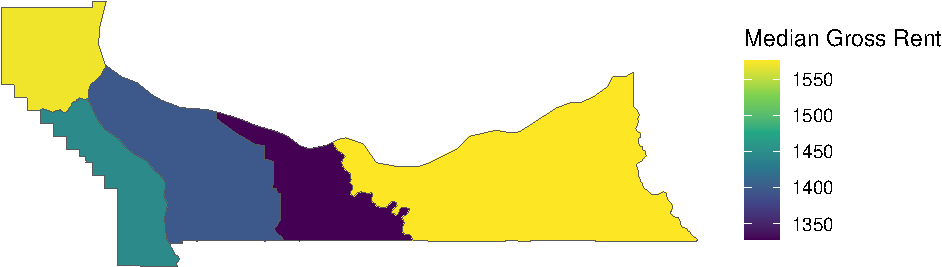
\includegraphics{lab06_files/figure-latex/unnamed-chunk-8-1.pdf}

\begin{Shaded}
\begin{Highlighting}[]
\NormalTok{tract }\SpecialCharTok{\%\textgreater{}\%}
  \FunctionTok{st\_as\_sf}\NormalTok{() }\SpecialCharTok{\%\textgreater{}\%}
    \FunctionTok{ggplot}\NormalTok{() }\SpecialCharTok{+}
    \FunctionTok{geom\_sf}\NormalTok{(}\FunctionTok{aes}\NormalTok{(}\AttributeTok{fill =}\NormalTok{ estimate)) }\SpecialCharTok{+}
    \FunctionTok{scale\_fill\_viridis\_c}\NormalTok{() }\SpecialCharTok{+}
    \FunctionTok{labs}\NormalTok{(}\AttributeTok{fill =} \StringTok{"Median Gross Rent"}\NormalTok{) }\SpecialCharTok{+}
    \FunctionTok{theme\_void}\NormalTok{()}
\end{Highlighting}
\end{Shaded}

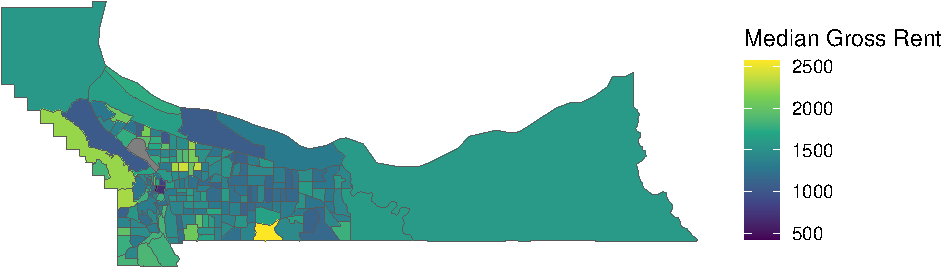
\includegraphics{lab06_files/figure-latex/unnamed-chunk-8-2.pdf}

\begin{Shaded}
\begin{Highlighting}[]
\NormalTok{block\_group }\SpecialCharTok{\%\textgreater{}\%}
  \FunctionTok{st\_as\_sf}\NormalTok{() }\SpecialCharTok{\%\textgreater{}\%}
    \FunctionTok{ggplot}\NormalTok{() }\SpecialCharTok{+}
    \FunctionTok{geom\_sf}\NormalTok{(}\FunctionTok{aes}\NormalTok{(}\AttributeTok{fill =}\NormalTok{ estimate)) }\SpecialCharTok{+}
    \FunctionTok{scale\_fill\_viridis\_c}\NormalTok{() }\SpecialCharTok{+}
    \FunctionTok{labs}\NormalTok{(}\AttributeTok{fill =} \StringTok{"Median Gross Rent"}\NormalTok{) }\SpecialCharTok{+}
    \FunctionTok{theme\_void}\NormalTok{()}
\end{Highlighting}
\end{Shaded}

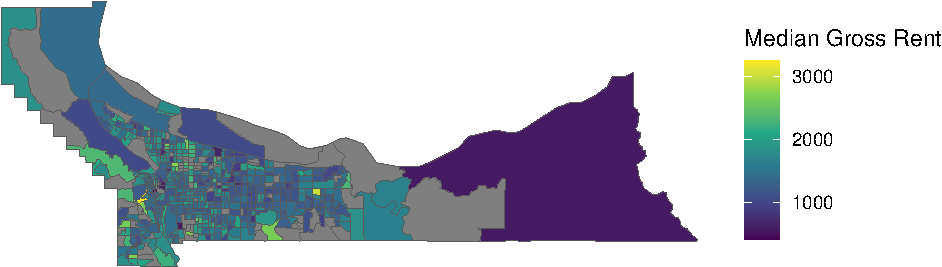
\includegraphics{lab06_files/figure-latex/unnamed-chunk-8-3.pdf}

\end{document}
